\documentclass[a4paper,10pt]{article}
\usepackage[american]{babel}
\usepackage[utf8]{inputenc}
\usepackage[left=2.5cm,top=2cm,right=2.5cm,nohead,nofoot]{geometry}
\usepackage{url}
\usepackage[colorinlistoftodos]{todonotes}
\usepackage{float}
\usepackage{hyperref}

\title{Artifical Intelligence Programming Paradigms\\Assignment 2}
\author{Antoine Carpentier}

\begin{document}

\maketitle

\section{Introduction}

In this assignment, we demonstrate the use of the Incremental Recruitment Language (IRL) framework to filter geometric forms by color. The primitive we introduce is named "filter-by-color". It can both filter an object set given a color and retrieve a color given a source set and a filtered set. We use an ontology in the primitive to retrieve the context and the colors. \\
We reuse some of the code from "irl-tutorial.lisp" to filter by shape and show several combinations of the two primitives. 
We also use the context defined in "irl-tutorial.lisp" and add colors to objects. \\
We introduce 3 color categories : red, green and blue and we think of a similarity measure to introduce continuous color values in RGB. \\
We also think of a way to chunk this primitive for composition and matching. \\
The code is available in the "assigment2.lisp" source file.

\section{Stand-alone use}

In \ref{fig:filter-color-1-evaluation}, we filter all red objects from the context using the primitive.

\begin{figure}[!h]
    \centering
    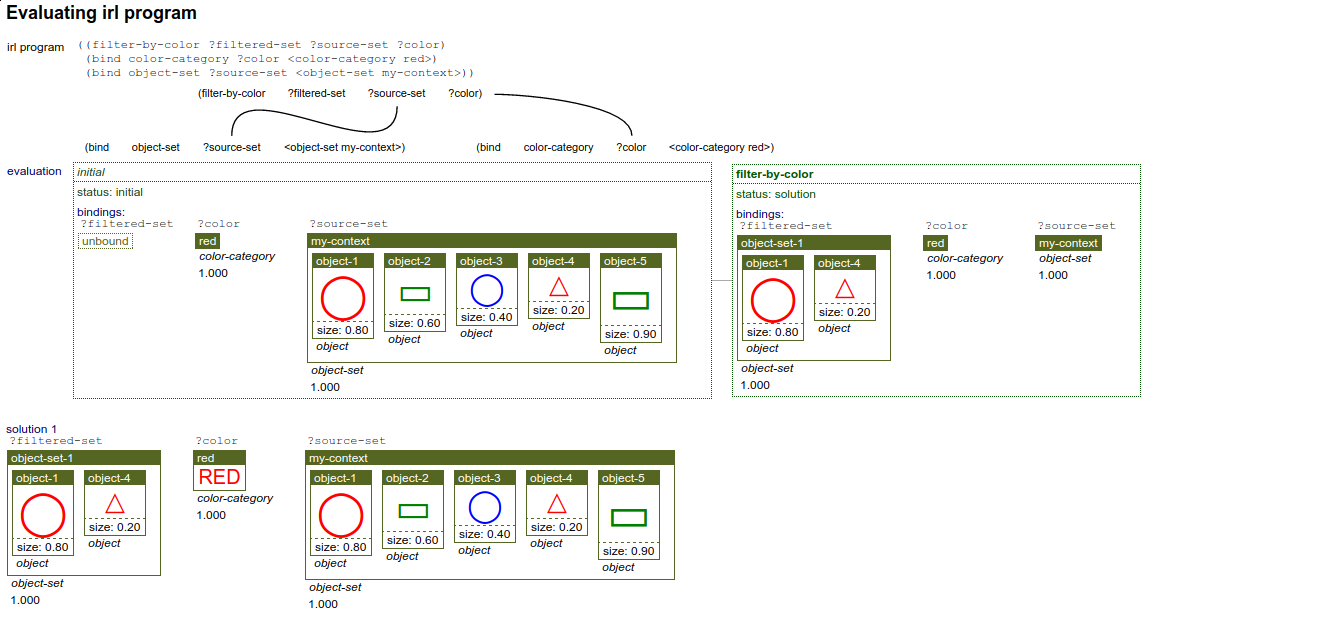
\includegraphics[width=1.0\textwidth]{filter-color-1-evaluation.png}
    \caption{Filter red objects from context}
    \label{fig:filter-color-1-evaluation}
\end{figure}

In \ref{fig:filter-color-2-evaluation}, we retrieve the red color from the context and a filtered set containing the red circle.

\begin{figure}[!h]
    \centering
    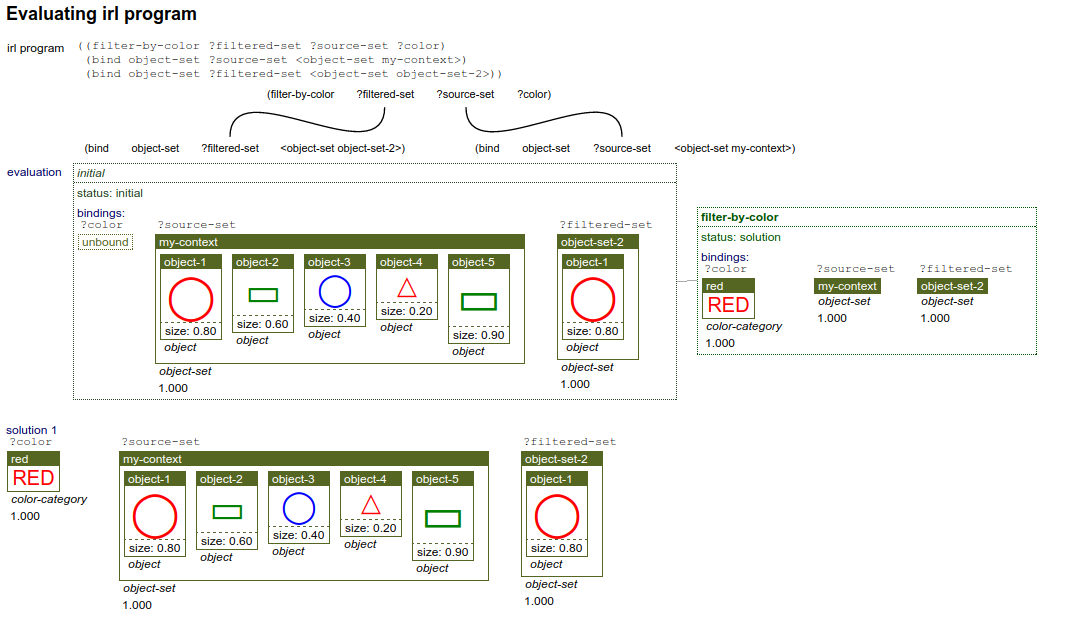
\includegraphics[width=1.0\textwidth]{filter-color-2-evaluation.png}
    \caption{Retrieve red color from context and red circle}
    \label{fig:filter-color-2-evaluation}
\end{figure}

In \ref{fig:filter-color-3-evaluation}, we try to retrieve yellow objects and there is no solution in this context.

\begin{figure}[!h]
    \centering
    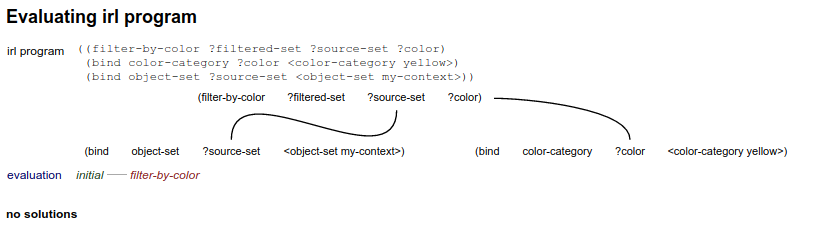
\includegraphics[width=1.0\textwidth]{filter-color-3-evaluation.png}
    \caption{Try to retrieve yellow objects}
    \label{fig:filter-color-3-evaluation}
\end{figure}

\section{Use in combination with shape}

In \ref{fig:filter-color-shape-1-evaluation}, we retrieve all red circle objects from the context using "filter-by-color" and "filter-by-shape".

\begin{figure}[!h]
    \centering
    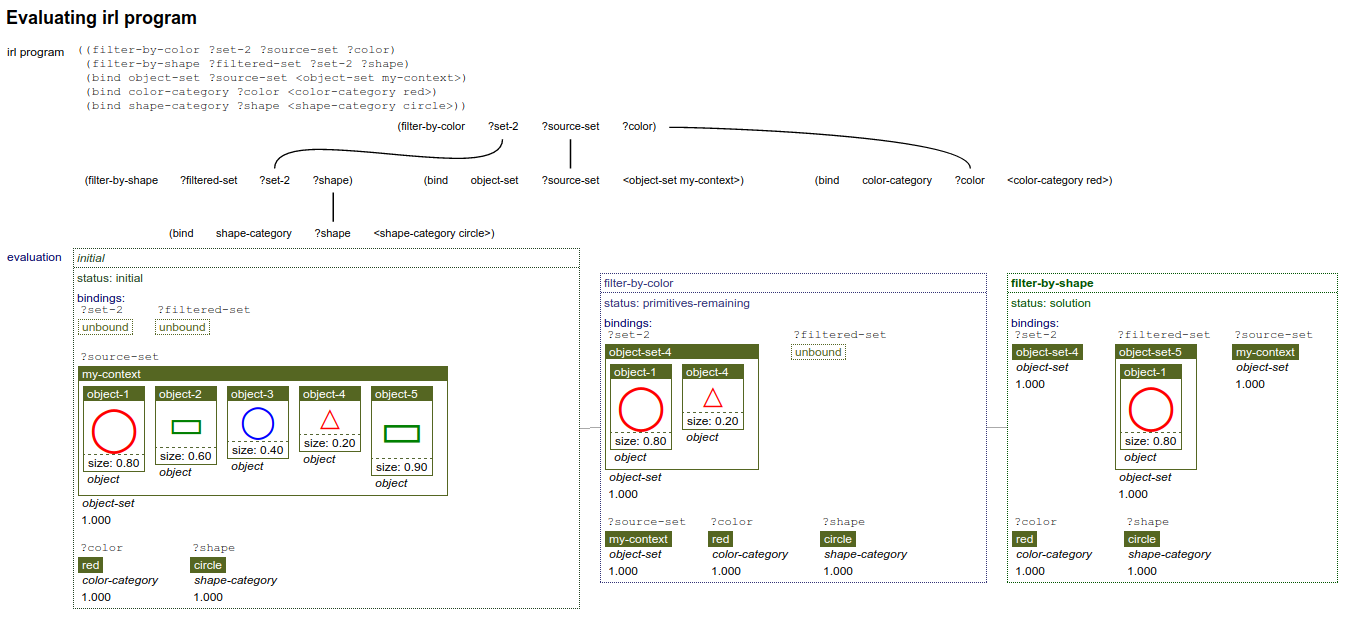
\includegraphics[width=1.0\textwidth]{filter-color-shape-1-evaluation.png}
    \caption{Filter red circle objects from context}
    \label{fig:filter-color-shape-1-evaluation}
\end{figure}

In \ref{fig:filter-color-shape-2-evaluation}, we retrieve the red color and the circle shape from the context and a filtered set containing the red circle.

\begin{figure}[!h]
    \centering
    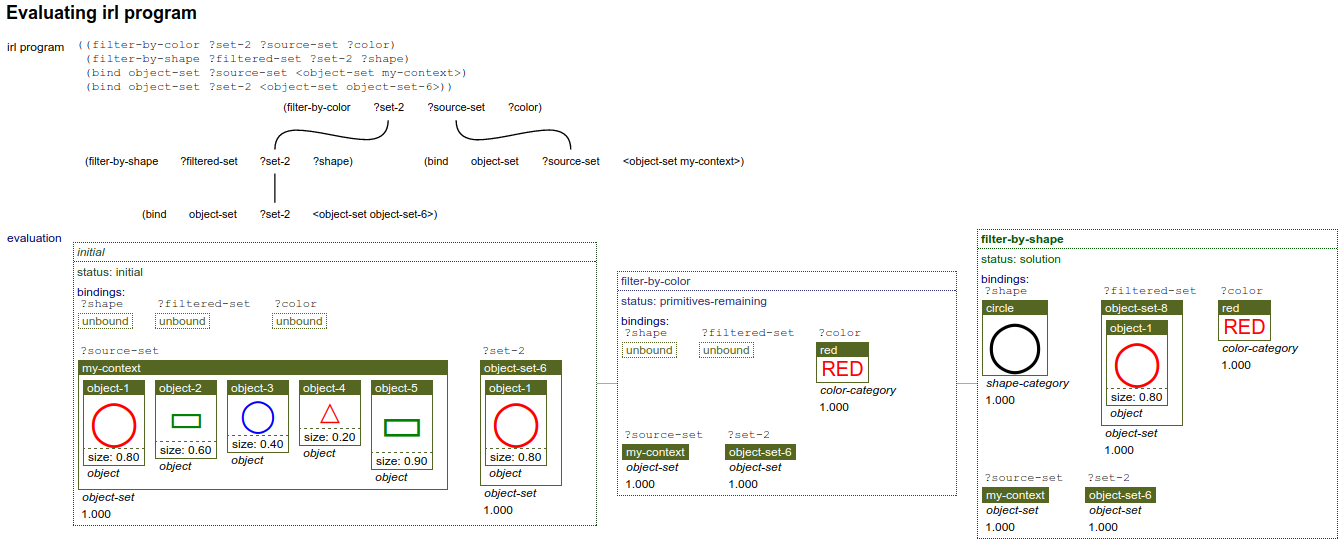
\includegraphics[width=1.0\textwidth]{filter-color-shape-2-evaluation.png}
    \caption{Retrieve red color and circle shape from context and red circle}
    \label{fig:filter-color-shape-2-evaluation}
\end{figure}

In \ref{fig:filter-color-shape-3-evaluation}, we try to retrieve red rectangles and there is no solution in this context.

\begin{figure}[!h]
    \centering
    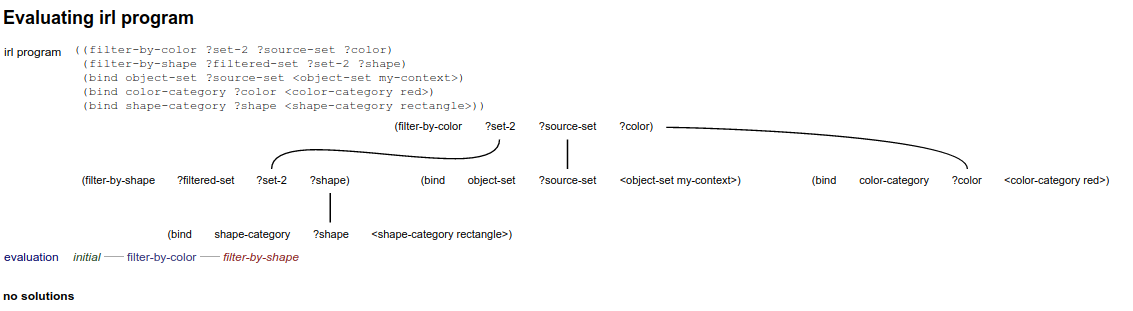
\includegraphics[width=1.0\textwidth]{filter-color-shape-3-evaluation.png}
    \caption{Try to retrieve red rectangles}
    \label{fig:filter-color-shape-3-evaluation}
\end{figure}

\section{Continuous color values}

In order to introduce continuous color values, we could code them as a triplet of RGB colors, each ranging from 0 to 1. The similarity measure would be the euclidian distance in the 3-dimensional space. Color categories would be defined as a triplet in the same way and in order to categorize a color in such a category, we would choose the category with the highest similarity.

\section{Chunk}

In \ref{fig:filter-color-chunk}, we use use a chunk to retrieve all objects of a given color. The chunk uses the primitives "get-context" and "get-color-category" to get data from the ontology.

\begin{figure}[!h]
    \centering
    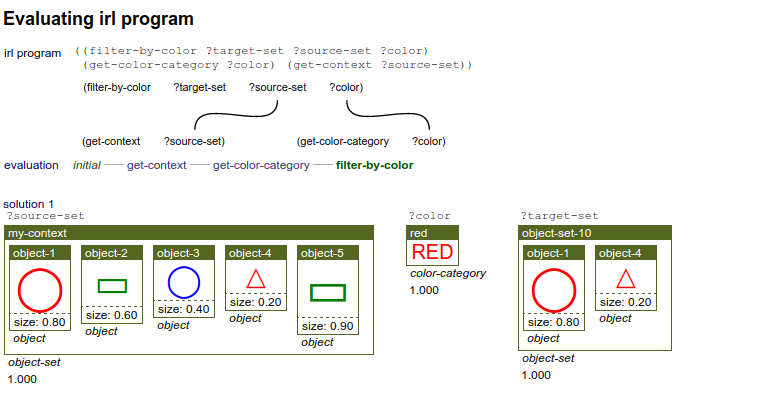
\includegraphics[width=1.0\textwidth]{filter-color-chunk.png}
    \caption{Retrieve red objects using a chunk}
    \label{fig:filter-color-chunk}
\end{figure}

\end{document}

